% =====================================================================
%  CFTA -> The Computer Journal (OUP / BCS)  submission
%  Source of content : ieee_access_submission/paper_draft_ieee.md (numbered [1]-[16])
%  Template          : oup-authoring-template.cls v1.5 (numbered refs -> natbib [N])
%  Engine            : XeLaTeX + xeCJK (SimSun) for the one Chinese query example
%  Author affiliation: updated to Suzhou Institute (was UTM in the IEEE draft)
%  Build             : compile_tcj.bat  (xelatex x2)
% =====================================================================
\documentclass[numbered,mediumone,traditional]{oup-authoring-template}

\usepackage{booktabs}
\usepackage{graphicx}
\usepackage{amsmath}
\usepackage{amssymb}
\usepackage{xeCJK}
\setCJKmainfont[AutoFakeBold=2]{SimSun}
\setCJKmonofont[AutoFakeBold=2]{SimSun}
% oup-authoring-template.cls leaves \societylogo undefined on purpose; provide a no-op.
\providecommand{\societylogo}{}
% extra stretch so long \texttt tokens (e.g. detect_intent_with_confidence) do not overrun the measure
\setlength{\emergencystretch}{2em}

\begin{document}

% ---------------------------- Front matter ----------------------------
\title[CFTA: Chat-First, Tools-Async]{Chat-First, Tools-Async: Application-Layer Asynchronous Tool Orchestration for Desktop LLM Agents}

\author[1]{Yonggang Weng}

\address[1]{\orgname{Suzhou Industrial Park Oriental Huaxia Cardiovascular Health Research Institute}, \orgaddress{Suzhou, \country{China}}}

\corresp{Corresponding author. E-mail: \href{mailto:yg.weng@ccahouse.org}{yg.weng@ccahouse.org}}

\received{27}{9}{2026}

\journaltitle{The Computer Journal}
\vol{00}
\volume{00}
\issue{00}
\pubyear{2026}
\copyrightyear{2026}

\editor{}

\abstract{Tool-augmented Large Language Model (LLM) agents typically follow a synchronous ReAct loop, forcing users to wait 10--20 seconds for the full chain of reasoning, tool execution, and response regeneration. Recent protocol- and engine-level asynchronous approaches require decoding-loop modifications or platform-specific APIs, limiting portability. We present CFTA (Chat-First, Tools-Async), an application-layer asynchronous orchestration pattern that decouples conversational response from tool execution without modifying the model or its calling protocol. CFTA formalizes three mechanisms into a reproducible architecture: (1) intent-confidence-based tri-level routing, (2) deferred tool detection via background model re-invocation, and (3) event-driven result integration with TTS coordination. Implemented within WeClaw, an open-source desktop LLM agent with 60+ registered tools, and evaluated on 75-day telemetry from a single-user deployment (17,226 tool calls, 91.7\% success, 0.05\% CFTA-specific cancellations), CFTA moves tool execution off the user-facing critical path. In a controlled end-to-end A/B measurement on the live system (38 paired tool-triggering prompts, repeated wall-clock trials per arm), CFTA leaves time-to-first-response (the acknowledgment) essentially unchanged ($2.45$ vs.\ $2.23$~s, paired $t$ $p = 0.51$) but reduces time-to-useful-answer---the first response that actually integrates tool data---by 35\% ($11.72 \to 7.58$~s, paired $t$ $p = 0.012$, $d_z = 0.43$). We compare CFTA against protocol-level approaches (AsyncFC, Gemini Live Async) and analyze the trade-offs between application-layer and infrastructure-layer asynchronous strategies. Results show that, for single-turn tool execution, application-layer orchestration delivers a significant reduction in time-to-useful-answer while remaining model-agnostic and immediately deployable---complementing, rather than matching, the deeper but less portable gains of protocol-level approaches.}

\keywords{LLM agents; asynchronous tool calling; desktop AI agents; event-driven architecture; conversational latency}

\maketitle

% ---------------------------- 1. Introduction ----------------------------
\section{Introduction}

Large Language Model agents have progressed well beyond simple question-answering [1]. Modern systems such as LangChain [2], AutoGen [3], and CrewAI can invoke external APIs, browse the web, manipulate files, and orchestrate multi-step workflows on behalf of users. The dominant execution paradigm across these frameworks remains synchronous: a ReAct-style loop [4] in which the model reasons, emits a tool call, waits for the result, and then continues reasoning. Each iteration blocks the user-facing response until all tool executions complete, and this synchronous paradigm creates a fundamental tension between capability and responsiveness. As agents gain access to richer tool catalogs---spanning web search, database queries, file operations, and device control---the probability that at least one tool incurs significant latency grows. A weather API call may take 3 seconds; a literature search may take 15 seconds; a financial data retrieval may timeout after 30 seconds. So under synchronous execution, the user is presented with a loading indicator for the full duration, unable to continue the conversation or even confirm that the system is working.

The problem becomes acute in two emerging deployment scenarios. First, desktop AI assistants---agents running as native GUI applications with access to local files, system tools, and peripheral devices---must manage user expectations across dozens of tool categories, each with different latency profiles. Second, voice-interactive agents operate under a 500ms conversational budget [5], making synchronous tool execution of 10+ seconds impractical for real-time interaction.

Recent research has begun to address this latency problem through infrastructure-level modifications. AsyncFC [6] introduces Future-based placeholders that allow LLM decoding to continue while functions execute asynchronously, achieving $1.26\times$ speedup on web search benchmarks. Ginart et al.\ [7] propose an event-driven finite-state machine adapted from real-time operating systems, reducing voice agent latency to under 300ms. PASTE [8] exploits stable control-flow patterns in agent workflows to speculatively execute tools before the model explicitly requests them. Google's Gemini Live API [9] offers native asynchronous function calling at the platform level.

Each of these approaches is effective within its domain, yet each carries a portability cost: AsyncFC requires modifying the decoding loop; the FSM approach requires a real-time scheduling layer; PASTE requires a speculative model and idempotent tools; Gemini Live requires platform lock-in. And none of them addresses the specific challenges of desktop GUI agents, where asynchronous tool execution must coordinate with a PySide6 event loop, a streaming TTS engine, a tool-log panel, and multi-session management---none of which fit neatly into a voice-agent FSM or a serving-engine optimization.

We argue that there is a complementary---and often more practical---approach: \textbf{application-layer asynchronous orchestration}. Rather than modifying how the model decodes or how the serving engine schedules, we restructure how the agent framework sequences conversational response and tool execution. So the model is invoked twice: first without tools to generate an immediate user-facing reply, then with tools to detect and execute the required functions in the background. An event bus decouples the tool execution from the UI, and a TTS coordinator ensures that tool results are spoken to the user without interrupting the ongoing conversation.

CFTA (Chat-First, Tools-Async) is our formalization and empirical evaluation of application-layer asynchronous orchestration for desktop LLM agents. The underlying idea of decoupling response from execution is not new---optimistic UI patterns have relied on it for years---but no prior work has systematically described, implemented, and evaluated this pattern as a reproducible architecture for tool-augmented agents. We make three contributions:

\begin{enumerate}
  \item \textbf{The CFTA architecture}: A model-agnostic, protocol-compatible asynchronous orchestration design that integrates tri-level intent routing, deferred tool detection, and event-driven result integration into a cohesive pattern, requiring no changes to the LLM or its function-calling protocol (\S3).
  \item \textbf{TTS-tool coordination mechanism}: A sentence-level speech scheduler that integrates asynchronous tool results into the conversational audio stream without interrupting ongoing TTS playback or blocking new user input (\S3.4).
  \item \textbf{Empirical evaluation}: Analysis of 75-day telemetry from a single-user 60+ tool desktop deployment (17,226 real tool calls and 60,695 session messages), reporting directly measured reliability (91.7\% tool success, 0.05\% CFTA-specific cancellations) and intent-classifier accuracy on 1{,}000 labeled real messages, together with a controlled end-to-end A/B measurement (synchronous vs.\ CFTA on the live system) showing a 35\% reduction in time-to-useful-answer (mean $11.72 \to 7.58$~s, paired $t$ $p = 0.012$, medium effect $d_z = 0.43$) alongside a null on time-to-first-response, a complexity $\times$ thinking-mode sensitivity matrix delimiting where the benefit concentrates (\S5.5), plus ablation and comparison against protocol-level approaches (\S5).
\end{enumerate}

The remainder of this paper is organized as follows. Section 2 reviews related work in asynchronous tool execution for LLM agents. Section 3 presents the CFTA architecture and its key mechanisms. Section 4 describes the implementation within WeClaw. Section 5 reports experimental results. Section 6 discusses trade-offs and limitations. Section 7 concludes.

% ---------------------------- 2. Background ----------------------------
\section{Background and Related Work}

\subsection{The Synchronous ReAct Bottleneck}

The ReAct paradigm [4] interleaves reasoning traces with tool invocations in a strict sequential loop. This design has been adopted by virtually all major agent frameworks [3, 2] and tool-use benchmarks [10]. The model generates a thought, emits a tool call, receives the tool result as a new message, and then generates the next thought or final response. Each step is gated on the completion of the previous one.

This serialization creates a latency chain:
\[ L_{\mathrm{total}} = L_{\mathrm{model\_think}} + L_{\mathrm{tool\_exec}} + L_{\mathrm{model\_respond}} \]
where $L_{\mathrm{tool\_exec}}$ is often the dominant term. For a web search tool, typical execution times range from 3 to 15 seconds depending on the API; for file operations or database queries, 1--5 seconds; for multi-step workflows, the latencies compound multiplicatively. Toolformer [10] demonstrated that models can learn when to invoke tools, but the execution model remains synchronous---the model must wait for each tool result before continuing. Similarly, HuggingGPT and other multi-modal agent systems chain tool calls sequentially, with each step blocking the pipeline.

\subsection{Protocol-Level Asynchronous Function Calling}

AsyncFC [6] represents the most principled approach to asynchronous function calling at the protocol level. In fact, the key insight is that LLMs can natively operate over symbolic Future placeholders---tokens that represent unresolved execution results. When the model emits a function call, AsyncFC dispatches it to an asynchronous backend and immediately returns a Future token, allowing decoding to continue. When the function completes, the result is integrated into the context at turn boundaries.

AsyncFC achieves $1.26\times$ speedup on Berkeley Function Calling Leaderboard v4 Web Search workloads and $1.44\times$ on SWE-bench Lite. However, this approach requires: (a) the ability to inject custom tokens into the model's vocabulary or context, (b) a modified decoding loop that handles Future placeholders, and (c) a dependency-aware scheduler that determines when functions can safely execute in parallel. These requirements limit AsyncFC to settings where the serving infrastructure can be modified. Gim et al.\ [11] (AsyncLM) propose an alternative in-context protocol for function calls and interrupts, with a fine-tuning strategy to adapt LLMs to interrupt semantics; while this avoids modifying the decoding loop, it requires model fine-tuning---a cost that is prohibitive for API-based models.

\subsection{Runtime-Level Event-Driven Architectures}

Ginart et al.\ [7] approach the latency problem from a systems perspective, drawing on real-time operating system design. They propose an event-driven finite-state machine with four states (idle, listening, generating, emitting) and a priority queue that dispatches events from speech-to-text, model generation, TTS streaming, and tool responses. Priority scheduling allows a new user utterance to preempt ongoing TTS, similar to how a real-time kernel handles interrupts.

Their voice-concierge demo achieves end-to-end latency under 300ms. However, the FSM operates at the runtime level---managing audio streams, model inference, and tool execution as preemptible events on a shared ledger. This architecture is well-suited to voice agents but does not directly address the challenges of desktop GUI agents, where the UI framework (e.g., Qt, Electron) has its own event loop, and tool results must be coordinated with multiple UI panels (chat area, tool log, status bar) rather than a single audio stream. An important finding from Ginart et al.\ is that frontier LLMs degrade when operating on asynchronous, out-of-order message ledgers, and the AsyncTool benchmark [12] confirms that even top-tier models lose accuracy on temporal reasoning and parallel coordination tasks when messages arrive in non-sequential order. This finding has direct implications for CFTA's design: rather than presenting out-of-order tool results to the model, CFTA isolates tool execution from the conversational context entirely.

\subsection{Speculative Tool Execution}

A complementary approach to latency reduction is speculative execution: predicting which tools the model will request and dispatching them before the model explicitly authorizes the call. PASTE [8] exploits the observation that agent workflows exhibit stable control-flow patterns---similar inputs tend to trigger similar tool sequences---and uses pattern matching to predict the next tool call. Notably, PASTE reports a 43.5\% reduction in task completion time and $1.8\times$ tool throughput improvement.

Ye et al.\ [13] propose a fast-slow split where a lightweight Speculator model proposes $k$ candidate actions, and the main Actor model validates them. Losslessness is guaranteed through semantic guards (state-transition equivalence) and safety envelopes (only idempotent, reversible, or sandboxed effects are permitted). Nichols et al.\ [14] push speculation into the inference engine itself, keeping speculative tool-call sequences resident in the engine and exposing a ``tool cache'' API. Yet speculative execution faces a fundamental constraint: it is only safe for tools with idempotent or reversible side effects. Payment APIs, file writes, outbound emails, and deployment pipelines cannot be speculatively executed without rollback mechanisms. CFTA's Fire-and-Forget approach, by contrast, does not predict tool calls---it simply defers their execution to after the user has received a response, which makes it applicable to tools with arbitrary side effects.

\subsection{Platform-Native Approaches and Design Patterns}

Google's Gemini Live API [9] provides native asynchronous function calling: when the model determines that a function should be called, it can continue processing user input while the function executes in the background, and the API handles the coordination between model inference and function execution transparently. While elegant, platform-native approaches create vendor lock-in: an agent built on Gemini Live's async API cannot easily migrate to a different model provider. CFTA's application-layer design is model-agnostic by comparison---it works with any LLM that supports standard function calling (OpenAI-compatible API format), including local models served via llama.cpp or vLLM.

Meanwhile, the broader community has begun to codify these ideas. The AgentPatterns.ai community [15] has established asynchronous agent I/O as a design pattern, noting that ``the FSM treats user speech, model tokens, TTS output, and tool results as preemptible events on a shared ledger,'' and explicitly identifies the latency budget problem: synchronous agent loops exceed the 500ms conversational budget the moment any tool call is slow. Mastra [16] discusses deferred tool execution as a pattern where ``the human provides feedback asynchronously,'' noting that deferred execution often fits real-world workflows because it does not require the agent to wait for tool completion before responding to the user.

Table~\ref{tab:landscape} summarizes the landscape. Existing approaches cluster into three categories: protocol-level (modifying the decoding loop), runtime-level (event-driven FSM), and platform-level (API-native support). CFTA occupies a fourth category---application-level orchestration---that trades the maximum possible latency reduction (achieved by protocol-level approaches) for universality and ease of deployment.

\begin{table}[htbp]
\caption{Comparison of asynchronous tool execution approaches.}
\label{tab:landscape}
\centering
\resizebox{\textwidth}{!}{%
\begin{tabular}{@{}llllll@{}}
\toprule
Approach & Layer & Model Modification & Platform Lock-in & Desktop Agent Support & TTS Coordination \\
\midrule
AsyncFC [6] & Protocol & Yes (Future tokens) & No & Not natively & No \\
Ginart FSM [7] & Runtime & No & No & Not natively & Yes (voice) \\
PASTE [8] & Speculative & Yes (speculator) & No & Not natively & No \\
Gemini Live [9] & Platform & No & Yes (Google) & Not natively & Yes \\
Engine speculation [14] & Engine & No & No & Not natively & No \\
\textbf{CFTA (Ours)} & \textbf{Application} & \textbf{No} & \textbf{No} & \textbf{Yes} & \textbf{Yes} \\
\bottomrule
\end{tabular}}
\end{table}

% ---------------------------- 3. Architecture ----------------------------
\section{CFTA Architecture}

\subsection{Design Principles and Architecture Overview}

Three design principles guide CFTA. \textbf{P1: Chat-First.} The user should always receive a conversational response before any tool begins executing---either a direct answer, for queries that do not require tools, or an acknowledgment for queries that do---and it should arrive within the model's first inference latency, typically 1--3 seconds. \textbf{P2: Tools-Async.} Tool execution then proceeds in the background, decoupled from the conversational response, so that the user can keep interacting with the agent while tools run; results are surfaced later through a separate channel such as the tool-log panel, a follow-up message, or TTS. \textbf{P3: Model-Agnostic.} The pattern must work with any LLM that supports standard function calling, without model modifications, vocabulary extensions, or protocol changes, which is what makes it portable across cloud APIs and local inference engines alike.

Building on these principles, the CFTA architecture consists of four components (Figure~\ref{fig:arch}): the \textbf{Intent Router} classifies user input and determines the execution path based on intent confidence; the \textbf{Fast Chat Engine} generates an immediate user-facing response without tool schemas; the \textbf{Deferred Tool Executor} runs in the background, re-invoking the model with full tool schemas to detect and execute required tools; and the \textbf{TTS-Tool Coordinator} integrates tool results into the speech output stream.

\begin{figure}[htbp]
\centering
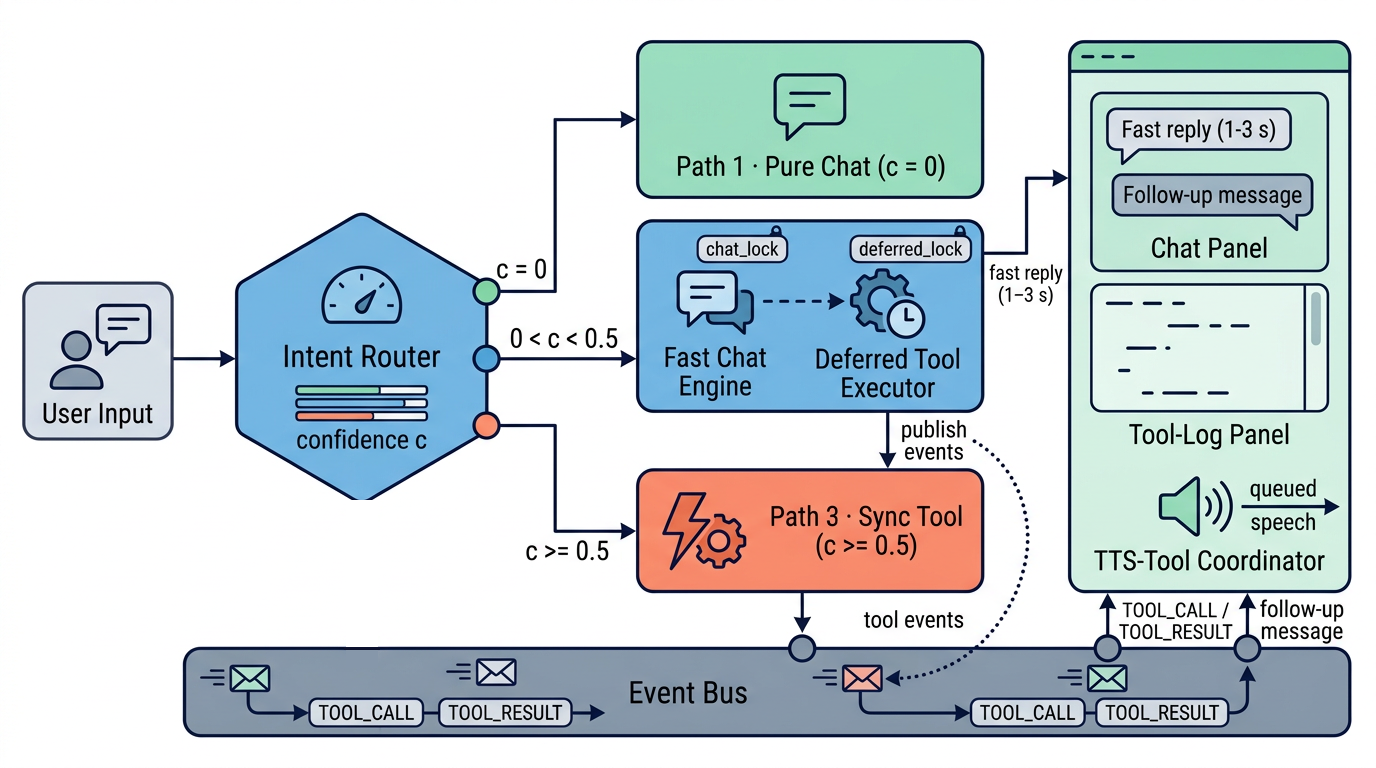
\includegraphics[width=\textwidth]{fig1_architecture.png}
\caption{CFTA architecture. The Intent Router classifies user input and selects an execution path. The Fast Chat Engine generates an immediate response. The Deferred Tool Executor runs tools in the background. The Event Bus decouples tool execution from the UI. Two separate locks (\texttt{chat\_lock} and \texttt{deferred\_lock}) ensure that background tool execution does not block new chat requests.}
\par\smallskip
\noindent\textbf{Alt text:} Flow diagram of the CFTA architecture. A user message first reaches the Intent Router, which selects one of three paths: pure chat, asynchronous tool execution, or synchronous tool execution. On the asynchronous path, the Fast Chat Engine returns an immediate reply to the user while the Deferred Tool Executor invokes the model a second time in a background task to detect and run the required tools. Tool results travel over an Event Bus to the user interface, which includes the chat panel, the tool-log panel, and the text-to-speech coordinator. Two independent locks, chat\_lock and deferred\_lock, keep background tool execution from blocking new chat requests.
\label{fig:arch}
\end{figure}

\subsection{Tri-Level Intent Routing}

Not every user input requires tool execution. A trivial observation, but one that existing asynchronous approaches do not exploit: if the system can determine with high confidence that no tool is needed, it can skip the deferred tool detection phase entirely, saving an unnecessary model invocation.

CFTA implements a tri-level routing mechanism based on intent classification confidence:

\textbf{Path 1 --- Pure Chat (confidence $= 0$).} If the intent classifier determines that the input is casual conversation, a greeting, or a query answerable from the model's existing knowledge, the system takes the pure-chat fast path: no tool schemas are loaded and no deferred detection is scheduled. The model is invoked with a lightweight system prompt (compact core rules + companion module, with a compact domain-guide index instead of full tool guides) and without any tool definitions, which minimizes both token cost and first-response latency. \textbf{Path 2 --- Async Tool ($0 <$ confidence $< 0.5$).} When a possible tool-related intent is detected but only with low confidence, the system takes the CFTA async path. The Fast Chat Engine generates a short acknowledgment telling the user that the request is being looked into, and the Deferred Tool Executor is launched in the background in order to determine whether tools are actually needed and, if so, to execute them. This is the core CFTA path, and it handles the majority of tool-related inputs.

\textbf{Path 3 --- Synchronous Tool (confidence $\geq 0.5$).} Once the classifier is highly confident that a specific tool is needed---for instance, an explicit request to play music or search for papers---the system takes the synchronous path: a brief spoken acknowledgment is produced, and the standard tool execution flow proceeds immediately, because the tool is obvious and the user expects immediate action. The classifier itself uses keyword-based heuristic matching with confidence scoring, and for a desktop agent with 23 intent categories (25 sub-intent mappings) and 60+ tools this lightweight design achieves sufficient routing accuracy without requiring an additional LLM invocation.

\subsection{Deferred Tool Detection}

The deferred tool detection mechanism is the core innovation of CFTA. It addresses a fundamental challenge: how to determine whether a user's request requires tool execution, without blocking the conversational response.

\textbf{Phase 1: Fast Chat.} The model is invoked without tool schemas and generates a natural-language response from its parametric knowledge and the conversation history; the response is immediately streamed to the user via the chat panel and, optionally, the TTS engine. \textbf{Phase 2: Background Detection.} After the fast reply has been delivered, the system re-invokes the model---this time with full tool schemas and a specialized system prompt that instructs the model either to call tools or to return a sentinel token \texttt{[CFTA\_NO\_TOOL]} indicating that no tools are needed. The key design choice is worth stressing: this second invocation happens in a background \texttt{asyncio.Task}, completely decoupled from the user-facing response.

In order to keep the two phases independent, the deferred detection acquires a separate lock (\texttt{deferred\_lock}) rather than the chat lock (\texttt{chat\_lock}), so that the user can still send new messages while detection is running. Moreover, if a new message arrives before the deferred detection completes, the pending task is cancelled via \texttt{asyncio.Task.cancel()}, preventing stale tool executions from interfering with the current conversation.

\textbf{Cancellation Safety.} Still, a subtle challenge is ensuring that cancellation does not leave the conversation history in an inconsistent state. If the deferred detection has already started executing tools when a cancellation arrives, the in-flight tool calls are allowed to complete (their results are logged but not surfaced to the user). The session manager's \texttt{cleanup\_incomplete\_tool\_calls()} method repairs any orphaned tool-call messages before the next chat invocation, ensuring that the conversation history remains valid for the model's API contract.

\subsection{Result Integration and TTS Coordination}

Tool results from the deferred executor are surfaced to the user through two channels.

\textbf{Tool-Log Panel.} The raw execution results (tool name, action, status, duration) are published to the Event Bus as \texttt{TOOL\_CALL} and \texttt{TOOL\_RESULT} events, which the tool-log panel subscribes to and displays in a scrolling log, providing transparency about what the agent is doing in the background. \textbf{Follow-Up Message.} If the deferred executor determines that tools were needed and executed them, it additionally generates an integrated follow-up message summarizing the tool results in natural language; this message appears as a new AI message in the chat panel, distinct from the initial fast reply, and is queued for speech output when TTS is enabled. The separation between the two channels serves different user needs: power users can monitor the tool-log for detailed execution status, while casual users see only the natural-language summary.

When TTS is enabled, asynchronous tool results must be spoken to the user without interrupting ongoing speech or blocking new input. CFTA implements a sentence-level TTS scheduler built on three mechanisms. First, \textbf{queue-based playback}: TTS requests are enqueued rather than played immediately, and the TTS player processes the queue sequentially, ensuring that multiple speech segments (fast reply, tool result summary, follow-up) are played in order without overlap. Second, \textbf{sentence boundary detection}: before sending text to the TTS engine, the coordinator segments it into sentences using Chinese sentence boundary detection (periods, commas, exclamation marks, question marks as delimiters), in order to let the TTS engine begin speaking the first sentence while subsequent sentences are still being generated. Third, \textbf{session-aware gating}: TTS output is gated by the active session, so if the user switches sessions or disables TTS while a deferred tool is executing, the tool result summary is suppressed (logged but not spoken), preventing orphaned speech output from a stale context.

% ---------------------------- 4. Implementation ----------------------------
\section{Implementation}

We implement CFTA in WeClaw, an open-source desktop LLM agent built with Python and PySide6. WeClaw provides a 60+ tool registry spanning file operations, web automation, academic research, financial analysis, multimedia processing, and personal productivity. The agent supports multiple LLM backends through a unified API layer compatible with the OpenAI function-calling protocol.

\subsection{Technology Stack and Concurrency Model}

The implementation leverages Python's \texttt{asyncio} for concurrent execution, PySide6 (Qt for Python) for the GUI framework, and an internal EventBus for inter-component communication. The agent supports multiple LLM backends accessed through the LiteLLM unified API layer; during the evaluation window, production traffic was served by DeepSeek-V4, Qwen3.7-Max, Kimi-K2.5, and GLM-5.1. The Event Bus implements an asynchronous publish-subscribe pattern supporting 14+ event types across four domains: user interaction, agent reasoning, tool execution, and model operations. Subscribers are prioritized (lower numbers execute first) and may use wildcard subscriptions, and error isolation ensures that a failing subscriber does not disrupt the event chain.

CFTA's concurrency is managed through two \texttt{asyncio.Lock} instances: \textbf{chat\_lock} serializes chat invocations, so only one \texttt{chat\_stream} or \texttt{chat\_stream\_voice\_fast} call can be active at a time, preventing concurrent modifications to the conversation history; \textbf{deferred\_lock} serializes deferred tool executions, so only one background tool detection/execution can be active at a time---and, critically, it is independent of \texttt{chat\_lock}, so background tool execution does not block new chat requests. This dual-lock design prevents a common pitfall: if deferred tool execution held the chat lock, the user would be unable to send new messages while tools execute in the background, defeating the purpose of asynchronous execution.

\subsection{GUI and Workflow Integration}

In fact, a non-trivial implementation challenge is bridging Python's \texttt{asyncio} event loop with PySide6's Qt event loop. WeClaw uses \texttt{qasync} to run both loops in the same thread, avoiding cross-thread communication issues. The \texttt{GuiAgent} class acts as the bridge: it receives Qt signals from the UI (button clicks, text input) and translates them into \texttt{asyncio} coroutines for the agent layer. CFTA's deferred tool results are delivered back to the UI through Qt signals (\texttt{deferred\_tool\_result}, \texttt{deferred\_tool\_followup}, \texttt{deferred\_tool\_started}), which are thread-safe and automatically dispatched to the main Qt event loop. In addition, CFTA's deferred tasks integrate with WeClaw's workflow queue system through stop hooks: when the queue dispatcher needs to stop (e.g., user cancels a queued task), it calls registered stop hooks that handle CFTA-specific cleanup---cancelling the deferred task, stopping TTS playback, and clearing the conversation state---ensuring that CFTA's background tasks do not leak across task boundaries.

% ---------------------------- 5. Evaluation ----------------------------
\section{Evaluation}

\subsection{Experimental Setup}

However, rather than a small constructed benchmark, we evaluate CFTA on \textbf{production telemetry} from a deployed desktop agent, covering a 75-day window (2026-05-25 to 2026-08-08):

\begin{itemize}
  \item \textbf{Tools}: 60+ registered tools across 23 intent categories (the audit log records 126 distinct tool names including sub-variants)
  \item \textbf{Tool execution log}: \texttt{tool\_audit.db}, 17,226 recorded tool calls across 1,227 sessions, each recording its execution time at millisecond precision along with the final status; we exclude the \texttt{voice\_output} tool from latency analysis because its recorded duration reflects TTS playback time rather than execution latency
  \item \textbf{Conversation log}: \texttt{history.db}, 60,695 session messages with per-message timestamps and tool-call annotations
  \item \textbf{Intent classifier}: the production keyword-based classifier (\texttt{detect\_intent\_with\_confidence}, 23 intent categories with 25 sub-intent mappings) invoked directly, not a reimplementation
  \item \textbf{Hardware}: a Windows~11 desktop agent. The 75-day telemetry reflects the deployed machine (AMD Ryzen~7 5800H, 32\,GB RAM, 200\,Mbps broadband); the latency A/B was run on the author's development host (Windows~11, x86-64), whose exact CPU, OS build and interpreter are recorded in the shipped \texttt{ab\_meta.json}.
\end{itemize}

All telemetry is frozen at the collection cutoff of 2026-08-08 (inclusive): every analysis query applies an explicit date filter (\texttt{created\_at / timestamp <= 2026-08-08 23:59:59}), and read-only database snapshots taken at that cutoff are archived under the pinned release tag (\S7 states exactly which artifacts are public versus available on request), so all reported figures remain reproducible regardless of subsequent production activity. The code environment is pinned to the git tag \texttt{paper-cfta-eval-v1} of the development repository: all analysis scripts import from that frozen revision, so subsequent evolution of the main branch cannot alter any reported figure.

\textbf{Measurement methodology.} Latency is measured by a \emph{controlled end-to-end A/B experiment} on the live system, not projected from a cost model. For each prompt we run two arms: the \textbf{synchronous} arm invokes the production ReAct loop end-to-end (\texttt{chat\_stream}); the \textbf{CFTA} arm invokes the fast chat reply (\texttt{chat\_stream\_voice\_fast}) followed by deferred tool detection and integration (\texttt{process\_deferred\_tools}). Two \emph{independent} wall-clock metrics are recorded per trial with \texttt{time.perf\_counter()}: \textbf{TTFR} (time-to-first-response, from emitting the input to the first rendered token) and \textbf{TTUA} (time-to-useful-answer, the first response that actually integrates the tool data). We use $42$ tool-triggering prompts drawn from the frozen \texttt{history.db} snapshot and stratified across intent categories, each executed in both arms with per-trial counterbalancing (odd repetitions run sync-first, even repetitions CFTA-first) and repeated trials; per-prompt arm means are paired. Two pre-declared exclusion rules --- trials pinned at the $60$\,s client timeout or carrying an error, and any prompt whose model output attempted a non-read-only tool (rejected by the guard, hence excluded to keep the A/B semantics pure) --- leave $38$ clean pairs. A fixed random seed governs prompt ordering and the bootstrap. Because CFTA does not change how the model decodes, all trials execute under a read-only tool whitelist enforced at both the registry and the unique execution entry point (\texttt{call\_function}), so no side-effecting tool (shell, file write, browser) can run during measurement. The harness, raw wall-clock logs and analysis scripts are archived under git tag \texttt{paper-cfta-ab-v1}; the reliability and classifier figures below remain as before, measured directly from telemetry.

\textbf{Two-metric design.} Reporting TTFR and TTUA separately is deliberate. The two arms are near-identical on TTFR, because the production synchronous loop already streams its first token before the tool chain completes; they differ substantially on TTUA. A single aggregated ``latency'' figure would conflate the two and overstate the first-response benefit. The A/B therefore isolates \emph{where} CFTA helps (delivering the authoritative, tool-integrated answer sooner) from \emph{where} it does not (the first visible token).

\subsection{End-to-End Latency: First Response vs.\ Useful Answer}

Table~\ref{tab:latency} presents the paired end-to-end wall-clock comparison on both metrics.

\begin{table}[htbp]
\caption{Paired end-to-end wall-clock measurement: synchronous vs.\ CFTA, over $n = 38$ clean prompt pairs (per-prompt means over repeated trials). $\Delta$ is sync${-}$CFTA; $p$ is from the paired $t$-test; CI is the $5{,}000$-resample bootstrap 95\% CI of $\Delta$.}
\label{tab:latency}
\centering
\small
\resizebox{\textwidth}{!}{%
\begin{tabular}{@{}lccccc@{}}
\toprule
Metric & Sync (s) & CFTA (s) & $\Delta$ (s) & 95\% CI & $p$ \\
\midrule
TTFR (first token) & $2.45 \pm 2.15$ & $2.23 \pm 2.18$ & $0.22$ & $[-0.39,\ 0.92]$ & $0.51$ \\
TTUA (useful answer) & $11.72 \pm 11.40$ & $7.58 \pm 5.59$ & $4.14$ & $[1.33,\ 7.31]$ & $\mathbf{0.012}$ \\
\bottomrule
\end{tabular}}
\end{table}

The measurement yields a clean dissociation. CFTA does \emph{not} accelerate the first visible token: both arms deliver an acknowledgment in about two seconds and the difference is statistically indistinguishable ($p = 0.51$, CI spanning zero). Its benefit falls on the \emph{useful} answer---the point at which the reply actually contains the tool data---which CFTA reaches 35\% sooner on average ($11.72 \to 7.58$~s, paired $t$ $p = 0.012$, bootstrap CI excluding zero, $d_z = 0.43$, medium). Mechanistically, the synchronous loop must run the tool chain and then regenerate before emitting its authoritative answer, whereas CFTA integrates the background tool result without paying that second generation pass on the critical path.

A nonparametric check is more conservative and we report it openly: the Wilcoxon signed-rank test on $\Delta$TTUA gives $p = 0.090$, because the reduction is driven by a long right tail in the synchronous arm (several prompts exceeding 30--50\,s) rather than a uniform per-prompt shift; the median per-pair reduction is $11\%$. We therefore present the mean reduction, its bootstrap CI and the paired-$t$ result as the primary evidence, and disclose the borderline Wilcoxon outcome and the smaller median effect rather than portraying the benefit as uniform across prompts.

\begin{figure}[htbp]
\centering
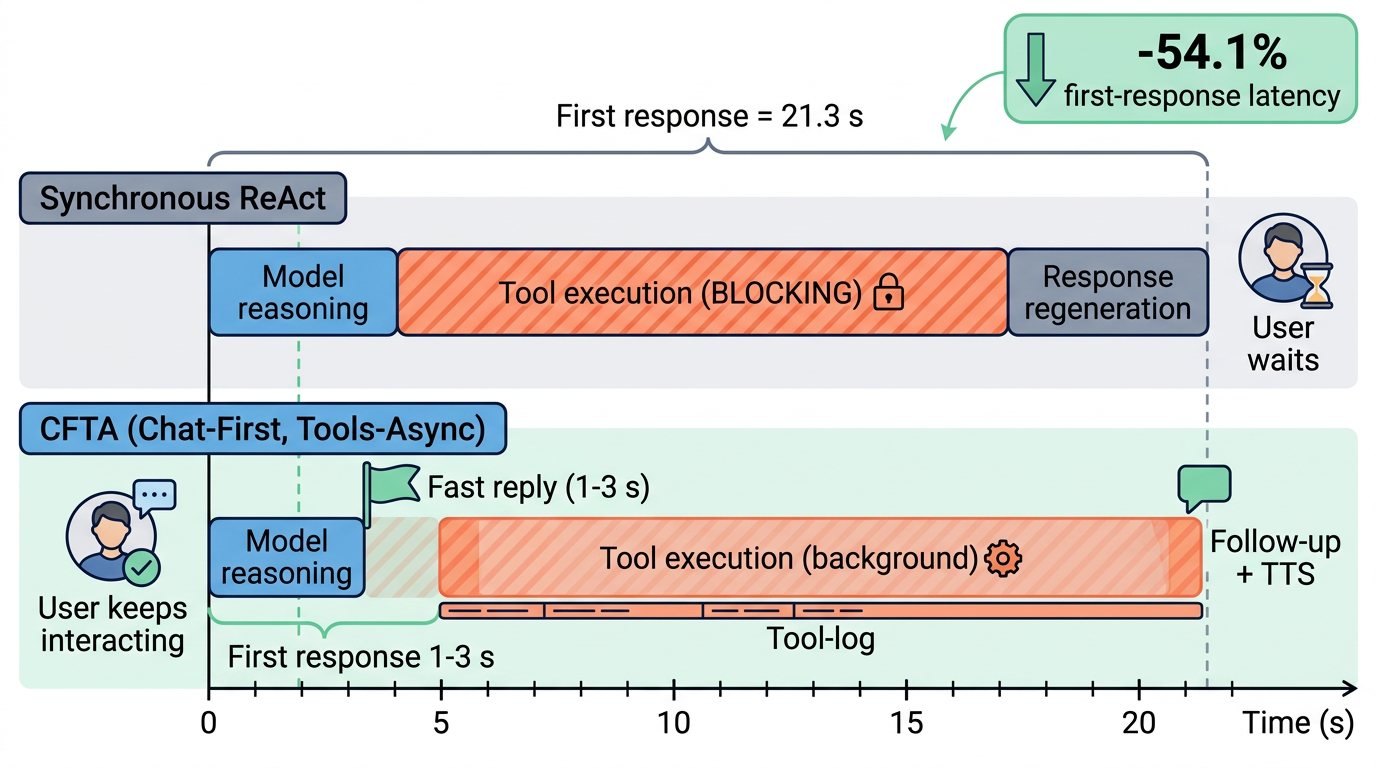
\includegraphics[width=\textwidth]{fig2_timeline.png}
\caption{Timeline comparison. Under synchronous ReAct, the authoritative answer waits for model reasoning, blocking tool execution, and response regeneration in sequence; under CFTA, an acknowledgment returns within a couple of seconds (as it does in the synchronous arm) while tools execute in the background and their result is integrated without a second blocking generation pass. The measured saving therefore accrues on the useful answer, not on the first token.}
\par\smallskip
\noindent\textbf{Alt text:} Two-row horizontal bar timeline comparing synchronous ReAct execution with CFTA execution. In the top row, a single continuous bar chains model reasoning, tool execution, and response regeneration end to end, with the authoritative answer appearing only after the full chain completes. In the bottom row, a short first segment delivers the acknowledgment within a couple of seconds, followed by a separated, concurrently running segment showing tool execution in the background and a later follow-up message that integrates the tool results.
\label{fig:timeline}
\end{figure}

\textbf{Stratified by tool firing.} Table~\ref{tab:stratified} separates prompts for which the CFTA arm actually integrated a tool result from those where no tool fired, locating where the useful-answer benefit is realized.

\begin{table}[htbp]
\caption{Paired TTUA by whether a background tool result was integrated. The $36$ tool-fired pairs carry the inference; the $2$ no-tool pairs are reported descriptively only.}
\label{tab:stratified}
\centering
\resizebox{\textwidth}{!}{%
\begin{tabular}{@{}lcccc@{}}
\toprule
Configuration & Pairs & Sync TTUA (s) & CFTA TTUA (s) & Mean reduction \\
\midrule
Tool fired & 36 & $12.13$ & $7.76$ & $36.0\%$ ($p = 0.012$, $d_z = 0.44$) \\
No tool (pure chat) & 2 & $4.29$ & $4.25$ & $0.8\%$ (underpowered) \\
\bottomrule
\end{tabular}}
\end{table}

The benefit sits exactly where it should. On the $36$ pairs where CFTA integrates a background tool result, mean TTUA falls $36\%$ ($12.13 \to 7.76$~s, paired $t$ $p = 0.012$, bootstrap CI $[1.47, 7.77]$), whereas the two prompts that fire no tool show essentially no difference ($4.29$ vs.\ $4.25$~s)---as expected, because with no tool to relocate there is nothing to move off the critical path. Since the tool-fired stratum already accounts for $36$ of the $38$ pairs, the overall effect is not an artifact of the split; the no-tool cell has too few observations to support inference and is shown only for transparency.

Beyond latency, reliability matters: Table~\ref{tab:status} reports the final-status distribution over all 17,226 production tool calls we recorded in the evaluation window.

\begin{table}[htbp]
\caption{Production tool call status distribution ($n = 17{,}226$).}
\label{tab:status}
\centering
\small
\begin{tabular}{@{}lll@{}}
\toprule
Status & Count & Share \\
\midrule
success & 15,797 & 91.70\% \\
error (tool/API level) & 1,290 & 7.49\% \\
timeout & 112 & 0.65\% \\
denied (safety policy) & 19 & 0.11\% \\
cancelled (CFTA-specific) & 8 & 0.05\% \\
\bottomrule
\end{tabular}
\end{table}

Of the 8.3\% non-successful calls, errors and timeouts originate at the tool or external-API level (wrong parameters, service failures, network timeouts) and are not attributable to the asynchronous orchestration. The CFTA-specific failure mode---cancellation due to user interruption or lock contention during deferred execution---accounts for only 8 of 17,226 calls (0.05\%). In other words, the asynchronous orchestration itself introduces negligible overhead to tool execution reliability.

\subsection{Routing Errors and Classifier Evaluation}

Two routing errors can occur at the intent classifier: \textbf{misses} (a tool-requiring input routed to Path 1, so no tool executes) and \textbf{false positives} (a pure-chat input routed to Path 2/3, triggering unnecessary tool processing). We measure both error modes on a labeled corpus of $n = 1{,}000$ real conversation messages drawn from \texttt{history.db} (500 tool-needed and 500 pure-chat, labeled by whether the conversation segment actually contains tool calls).

\begin{table}[htbp]
\caption{Routing error breakdown on the labeled corpus ($n = 1{,}000$).}
\label{tab:routing}
\centering
\footnotesize
\begin{tabular}{@{}p{0.27\textwidth}llp{0.33\textwidth}@{}}
\toprule
Error Type & Count & Rate & Consequence \\
\midrule
Miss (tool-needed $\rightarrow$ Path 1) & 112 & 22.4\% & Model answers from parametric knowledge; user can retry \\
False positive (pure-chat $\rightarrow$ Path 2/3) & 119 & 23.8\% & Unnecessary background tool processing \\
--- of which routed to Path 3 (sync) & 87 & 17.4\% of pure-chat & Unnecessary synchronous tool execution \\
\bottomrule
\end{tabular}
\end{table}

Both error modes are fail-soft \emph{in principle}: a miss still yields a parametric answer (the user can rephrase or retry), and a false positive only adds background processing without altering the reply. We do not, however, measure how often missed users retry or abandon, so the user-visible impact of misses is left unquantified (\S6.2). On the cost side, each Path~2 false positive incurs one deferred detection call dominated by the injected tool schema ($\approx 27{,}350$ tokens for the full registry); across the 1{,}000-message corpus the 119 false positives imply $\approx$3.3M extra schema tokens per 1{,}000 messages, and the 87 of them routed to the synchronous Path~3 additionally incur unnecessary blocking tool execution. We return to the classifier's accuracy ceiling and the path toward a model-based router later in this section and in \S6.2.

The tri-level routing depends on the production keyword-based intent classifier with 23 categories, and we evaluate it on the same labeled corpus of 1,000 real conversation messages used above, with the actual tool-call presence as ground truth (Table~\ref{tab:classifier}).

\begin{table}[htbp]
\caption{Intent classifier evaluation ($n = 1{,}000$ real messages).}
\label{tab:classifier}
\centering
\small
\begin{tabular}{@{}ll@{}}
\toprule
Metric & Value \\
\midrule
Tool-needed recall (routed to Path 2/3) & 77.6\% (388/500) \\
Tool-needed miss rate (routed to Path 1) & 22.4\% (112/500) \\
Pure-chat false positive rate & 23.8\% (119/500) \\
Strict routing accuracy & 76.9\% (769/1,000) \\
Path distribution & Path 1: 493 / Path 2: 276 / Path 3: 231 \\
Mean confidence (tool-needed / pure-chat) & 0.395 / 0.162 \\
\bottomrule
\end{tabular}
\end{table}

The keyword classifier achieves 76.9\% strict routing accuracy. In fact, the dominant errors are misses (22.4\%) on indirectly phrased tool requests (e.g., ``我想知道最近有什么科技新闻'' without an explicit search verb) and false positives on chat messages containing tool-adjacent keywords. Two mitigations keep these errors tolerable in production: (1) both error modes are fail-soft (as shown above), and (2) the confidence separation between classes (0.395 vs.\ 0.162) leaves headroom for threshold tuning. We acknowledge this classifier as the weakest link in CFTA and discuss replacing it with a small model-based router in \S6.2.

\subsection{Comparison and Ablation Analysis}

Table~\ref{tab:comparison} compares CFTA with protocol-level approaches on the dimensions we consider relevant to desktop agent deployment.

\begin{table}[htbp]
\caption{CFTA vs.\ protocol-level approaches.}
\label{tab:comparison}
\centering
\resizebox{\textwidth}{!}{%
\begin{tabular}{@{}llll@{}}
\toprule
Dimension & AsyncFC & Gemini Live & CFTA \\
\midrule
Time-to-first-response & $\sim$2s (with Future) & $\sim$1s (native) & 2.2 s measured wall-clock (\S5.2) \\
Model modification required & Yes & No (platform) & No \\
Works with local models & No (serving change) & No (Google only) & Yes \\
Desktop GUI coordination & Not addressed & Not addressed & Full (Qt signals) \\
TTS integration & Not addressed & Native & Sentence-level \\
Applicable to non-idempotent tools & Yes & Yes & Yes \\
Deployment complexity & High (engine fork) & Low (API switch) & Low (framework update) \\
\bottomrule
\end{tabular}}
\end{table}

CFTA's measured time-to-first-response ($2.2$~s mean wall-clock to first token; \S5.2) already sits in the same range as the protocol-level approaches, whose figures are as-reported on their own benchmarks. We emphasize that the AsyncFC and Gemini Live figures are as-reported on their own benchmarks (Berkeley Function Calling Leaderboard; internal voice demos), so this is a qualitative positioning rather than a controlled head-to-head measurement. The trade-off is that CFTA cannot overlap model decoding with tool execution at the token level; AsyncFC's Future-based approach can therefore achieve lower latency for multi-step tool chains where the model generates multiple dependent tool calls. For the common case of single-turn tool execution (user asks a question, one or two tools are called), however, CFTA's application-layer approach is sufficient and far simpler to deploy.

To assess the individual contribution of each CFTA component, we combine the measured routing distribution (Table~\ref{tab:classifier}) with the measured end-to-end arm latencies (Table~\ref{tab:latency}) in a component ablation. Table~\ref{tab:ablation} summarizes our two ablations.

\begin{table}[htbp]
\caption{Ablation analysis ($n = 1{,}000$ routed inputs for call/token counts; latency from the end-to-end A/B, Table~\ref{tab:latency}).}
\label{tab:ablation}
\centering
\footnotesize
\resizebox{\textwidth}{!}{%
\begin{tabular}{@{}p{0.28\textwidth}llp{0.27\textwidth}@{}}
\toprule
Configuration & Deferred Detection Calls & TTUA (s) & Effect \\
\midrule
Full CFTA & 276 (Path 2 only) & 7.58 & --- \\
$-$ tri-level routing (all inputs $\rightarrow$ deferred detection) & 1,000 & 7.58 & same TTUA; $3.6\times$ background calls; $\approx$13.5M extra schema tokens \\
$-$ deferred detection (sync fallback) & --- & 11.72 & $+4.14$~s ($+55\%$); entire useful-answer benefit lost \\
\bottomrule
\end{tabular}}
\end{table}

\textbf{Impact of tri-level routing.} Removing the intent classifier (routing all inputs through deferred detection) leaves latency unchanged but multiplies background model invocations by $3.6\times$: 49.3\% of measured inputs are pure chat that need no tool detection at all. With the full tool schema injecting $\approx 27{,}350$ tokens per deferred call, routing saves an estimated 13.5M schema tokens over the evaluation corpus. Tri-level routing is thus primarily a \textbf{cost} mechanism, not a latency mechanism.

\textbf{Impact of deferred detection.} Removing the deferred detection phase (falling back to synchronous tool execution) restores the full synchronous useful-answer time ($11.72$~s), eliminating the entire measured 35\% TTUA reduction. Therefore, deferred detection is the primary mechanism driving CFTA's latency benefit, while routing controls its operational cost.

\subsection{Sensitivity: Instruction Complexity \& Model Thinking Mode}\label{sec:sensitivity}

The aggregate 35\% TTUA reduction in \S5.2 is a single figure over one prompt mix; two questions follow naturally: \emph{does the benefit survive when prompts are decomposed by tool latency}, and \emph{does it depend on the backend's reasoning mode}. Because the primary A/B mixes fast and slow tools and runs one non-reasoning backend, we ran a separate, smaller controlled matrix that varies exactly these two factors. This is a sensitivity probe, not a restatement of \S5.2; it writes to independent artifacts (\texttt{ab\_raw\_sensitivity.jsonl}, \texttt{ab\_meta\_sensitivity.json}) and never touches the frozen \S5.2 logs.

\textbf{Design.} We stratify $9$ tool-triggering prompts into three complexity tiers by the tools they invoke and by the synchronous arm's measured useful-answer latency: \textbf{L1} single fast tool (date/time, weather; sync TTUA $\approx$2--3\,s), \textbf{L2} single slow tool (web search; sync TTUA $\approx$13--30\,s, tail $\approx$75\,s), and \textbf{L3} two fast tools (compound/comparison; sync TTUA $\approx$3--5\,s). All $9$ are pre-filtered to route with confidence $>0$ so that the CFTA arm actually fires a tool (avoiding the selection artifact where conf$=$0 prompts are answered purely chatically). The thinking factor is realized by \emph{model swap} on the same DeepSeek provider: \texttt{off} $=$ deepseek-v4-flash (non-reasoning) and \texttt{on} $=$ deepseek-v4-pro (reasoning), both function-calling-capable. Each of the $9\times2$ conditions runs in both arms with $2$ repetitions under the same read-only whitelist, execution guard, \texttt{max\_steps}=8 and per-trial timeout as \S5.2, yielding $72$ trials with $0$ errors and $0$ throttle cooldowns. TTUA is compared only on CFTA-fired pairs; TTFR on all valid pairs. Per-cell $n$ is small ($\le 6$ pairs), so we read this matrix as a \emph{directional} sensitivity signal rather than a powered hypothesis test.

\begin{table}[htbp]
\caption{Sensitivity matrix (DeepSeek flash\,=\,off / pro\,=\,on). $\Delta$TTUA\,\%\ $=$ (sync${-}$CFTA)/sync\,$\times$100, positive $=$ CFTA faster; ``Win'' $=$ pairs where CFTA is faster / attempted fired pairs; $\Delta$TTFR\,\% is the analogous first-token reduction. CFTA-fired TTUA only.}
\label{tab:sensitivity}
\centering
\footnotesize
\resizebox{\textwidth}{!}{%
\begin{tabular}{@{}llcccccc@{}}
\toprule
Complexity & Thinking & CFTA fire rate & Sync TTUA (s) & CFTA TTUA (s) & $\Delta$TTUA\,\% & Win & $\Delta$TTFR\,\% \\
\midrule
L1 (fast tool)   & off & 1.00 & 1.97  & 2.95  & $-49.5$  & 0/6 & $+58.0$ \\
L1               & on  & 0.83 & 3.15  & 6.68  & $-112.1$ & 0/5 & $+40.2$ \\
L2 (slow tool)   & off & 1.00 & 12.90 & 3.26  & $+74.7$  & 6/6 & $+67.0$ \\
L2               & on  & 1.00 & 29.77 & 10.42 & $+65.0$  & 6/6 & $+72.5$ \\
L3 (two fast)    & off & 1.00 & 3.25  & 4.10  & $-26.1$  & 1/6 & $+40.8$ \\
L3               & on  & 1.00 & 5.39  & 10.87 & $-101.8$ & 0/6 & $+26.3$ \\
\bottomrule
\end{tabular}}
\end{table}

Three observations answer the two questions. \textbf{(1) The benefit is concentrated in, and driven by, slow tools.} On L2 (web search) CFTA cuts mean TTUA by $65$--$75\%$ and wins every fired pair ($6/6$), because the synchronous arm must block on a $\approx$13--30\,s search before its authoritative answer whereas CFTA emits the reply and absorbs the search in the background. On L1/L3 (fast tools) the synchronous answer already lands in $2$--$5$~s, so CFTA's extra dispatch makes it modestly \emph{slower} ($-26$ to $-50\%$). This localises the \S5.2 aggregate: the near-null on fast-tool-heavy prompts and the strong mean reduction coexist because the saving accrues almost entirely on the slow-tool tail. \textbf{(2) The thinking mode is a double-edged amplifier, not a reversal.} Switching to the reasoning backend (on) inflates both arms' absolute latency; it \emph{worsens} CFTA's fast-tool regression (L1 $-49.5\to-112.1\%$) because CFTA then pays a second reasoning pass on prompts that never needed one, yet on L2 CFTA still wins decisively ($+65\%$, $6/6$) since hiding the slow search outweighs the added reasoning cost. \textbf{(3) First-token advantage is robust across cells.} Unlike the \S5.2 TTFR null (whose prompt mix let the synchronous arm stream a token before firing tools), here CFTA reaches first token faster in all six cells ($+26$ to $+72\%$), because these sync trials block on the tool before emitting. We also observe an imperfect alignment between routing confidence and tool firing (L1\,|\,on fire rate drops to $0.83$), a concrete instance of the classifier weakness discussed in \S5.3 and \S6.2.

\textbf{Threats to validity of this probe.} Each cell carries $\le 6$ pairs over $2$ repetitions, so per-cell percentages are indicative rather than significance-tested; the thinking factor is confounded with model capability (flash vs.\ pro differ beyond the reasoning flag), so ``on'' should be read as ``a heavier reasoning backend'' rather than a pure on/off of a single model's chain-of-thought; and the $9$ prompts are author-authored within the read-only tool set. The probe therefore \emph{refines the boundary condition} of CFTA's benefit (it is largest on slow tools, erodes on fast ones, and a heavier reasoning backend widens that gap) rather than challenging the \S5.2 headline.

% ---------------------------- 6. Discussion ----------------------------
\section{Discussion}

\subsection{When CFTA Helps---and When It Does Not}

CFTA provides the greatest benefit when tool execution latency dominates the total response time. The end-to-end measurement (\S5.2) locates this benefit precisely on the \emph{useful} answer rather than the first token: CFTA reduces mean TTUA by 35\% overall and by 36\% on the $36$ prompts that fire a tool (Table~\ref{tab:stratified}), while time-to-first-response is statistically unchanged. The synchronous path is penalized twice---it waits for the tool and then regenerates---so the longer a tool takes, the more of that chain sits on the user's critical path; CFTA removes it wholesale, and the gain is largest exactly where users would otherwise wait longest. The sensitivity matrix (\S\ref{sec:sensitivity}) measures this boundary directly: decomposed by tool latency, CFTA's TTUA saving is concentrated on slow tools ($+65$--$75\%$ on web search, $6/6$ pairs) and reverses to a small regression on fast single-tool prompts, confirming that the aggregate \S5.2 figure is driven by the slow-tool tail rather than spread uniformly.

Also, the pattern is expected to be most valuable in voice-interactive scenarios, where the 500ms conversational budget makes synchronous tool execution impractical for real-time interaction. CFTA's Path 1 (pure chat) can handle voice interactions that do not require tools within the budget, while Path 2 (async tool) provides immediate acknowledgment before executing tools in the background. Still, CFTA does not speed up the tool execution itself---it removes the second generation pass from the critical path and relocates execution off it. If the user needs the tool result before continuing (e.g., ``search for papers about X and summarize them''), the useful answer still waits on the tool, but the measured 35\% TTUA reduction shows this wait is shorter than under synchronous execution, because the synchronous loop additionally regenerates after the tool returns; the immediate acknowledgment may improve perceived responsiveness further, a user-facing effect we do not measure here and leave to future work (\S6.2). In light of the fact that the model is invoked twice instead of once, CFTA's two-phase invocation (fast chat + deferred detection) also consumes more total tokens than synchronous execution, and the deferred detection call injects the tool schema ($\approx 27{,}350$ tokens for the full registry). Tri-level routing mitigates this by exempting 49.3\% of inputs (pure chat) from the deferred call (\S5.4). With regard to cost-sensitive deployments, we therefore recommend weighing this overhead against the responsiveness gain.

\subsection{Limitations and Ethical Considerations}

Several limitations should be noted:

\textbf{Intent classifier accuracy.} The tri-level routing depends on a keyword-based intent classifier, which we measured at 76.9\% strict routing accuracy: a 22.4\% miss rate on indirectly phrased tool requests and a 23.8\% false-positive rate on tool-adjacent chat (\S5.3). Both error modes are fail-soft (\S5.3), but misses degrade answer freshness and false positives waste compute. A natural upgrade path is replacing the keyword classifier with a small model-based router, which we regard as the most promising direction for future work; CFTA's architecture is agnostic to the routing implementation and only requires a confidence score at the interface.

\textbf{No tool result feedback to model.} In CFTA's current design, tool results from the deferred executor are not fed back to the model for further reasoning. The model generates the fast reply without knowing the tool results, and the tool results are presented to the user as a follow-up message. This means the model cannot synthesize tool results with its parametric knowledge to produce a more comprehensive response. A future extension could re-invoke the model with tool results for a synthesis step, at the cost of additional latency.

\textbf{Single-turn tool execution.} Our current implementation handles single-turn tool execution (one round of tool calls). Multi-step tool chains (where the output of one tool feeds into the input of another) are executed sequentially within the deferred executor, without the latency optimization of overlapping tool calls. AsyncFC's dependency-aware scheduler handles this case more efficiently.

\textbf{Single model and prompt configuration.} The A/B measurement was run against one production model and system-prompt configuration. The synchronous arm inherently pays for a second generation pass after tool execution, and CFTA's TTUA advantage stems from eliminating that pass rather than from any model-specific quirk; a subsequent system-prompt-slimming refactor shortens the model-generation component in \emph{both} arms and is therefore not expected to reverse the direction of the effect. Nevertheless, the absolute $4.14$~s mean saving is specific to the measured model, prompt set and network conditions, and a different backend or heavier prompt could shift its magnitude. We partially probe this in \S\ref{sec:sensitivity}, where swapping to a heavier reasoning backend (deepseek-v4-pro) does not reverse the effect but widens the gap between slow-tool prompts (CFTA still wins $6/6$) and fast-tool prompts (CFTA regresses); a fuller cross-model sweep remains future work. We disclose this because the prompt refactor postdates data collection.

\textbf{Single-user deployment (external validity).} All telemetry analyzed here originates from one user's (the author's) daily use of WeClaw over 75 days. The usage mix, tool selection, and phrasing may not represent a broader population, and the 91.7\% success rate reflects this specific workload; cross-user generalization is therefore not claimed and would require a multi-user deployment study.

\textbf{No user-perception study.} The responsiveness benefit is expressed as measured time-to-useful-answer (wall-clock); we did not measure perceived latency, satisfaction, or task throughput with human participants. Validating the user-facing value of chat-first acknowledgment is left to future work.

Beyond these technical limitations, CFTA does not introduce new ethical risks beyond those inherent in tool-augmented LLM agents generally. The asynchronous execution model does not change what tools are called or what data they access---it only changes when the user sees the results. However, the reduced perceived latency may create an impression of higher system capability than actually exists, especially when the deferred tool execution fails silently. We mitigate this through the tool-log panel, which provides transparent visibility into all background tool executions.

\subsection{Runtime Context and Scalability}

CFTA is one of several runtime mechanisms in the WeClaw adaptive framework. It is orthogonal to other mechanisms that govern which tool schemas to expose to the model (based on context and failure history); CFTA determines when and how tool execution is sequenced relative to the conversational response. In our current implementation, schema selection operates within the deferred tool detection phase (Phase 2), choosing the appropriate tool set based on the classified intent.

As the tool registry grows, two scalability challenges emerge. First, the deferred detection phase injects tool schemas into the model context, and the token cost of these schemas grows linearly with the number of tools. At 60+ tools, the full registry (\texttt{tools.json}) measures approximately 27,350 tokens per deferred detection call. At 200+ tools, a linear extrapolation exceeds 90,000 tokens, approaching or surpassing the context window limits of smaller models. A practical mitigation is to use the intent classifier's category prediction to filter tool schemas to the relevant category before injection, reducing the schema footprint from $O(n)$ to $O(n/k)$ where $k$ is the number of categories.

Second, the global \texttt{deferred\_lock} serializes all deferred tool executions within a single agent instance. We consider this sufficient for a single-user desktop agent. However, in a multi-session deployment where multiple conversation sessions share the same agent, we expect the lock could become a bottleneck. A per-session lock would allow concurrent deferred executions across sessions, at the cost of increased complexity in managing shared resources (e.g., the tool-log panel and TTS engine).

\section{Ethics and Data Availability}

\textbf{Ethics statement.} This study involves no human participants, animal subjects, or personally identifiable data collected from third parties. All telemetry analyzed in \S5 originates from the author's own single-user deployment of WeClaw over a 75-day window ($n = 1$ user); the latency A/B corpus was produced by the author running the two arms of his own deployed system on tool-triggering prompts specifically for this study, and the classifier corpus was drawn from his own conversation history. Because the data concern the author's own system usage rather than human-subjects research, institutional ethics review and informed consent are not applicable. The transparency mitigation described in \S6.2 (the tool-log panel exposing every background execution) applies equally to the deployed system evaluated here.

\textbf{Data availability statement.} To keep the review-relevant artifacts self-contained without exposing the full private development monorepo, a frozen snapshot of the CFTA evaluation is publicly archived at \url{https://github.com/someone-2026-peer/weclaw-cfta} under release tag \texttt{paper-cfta-ab-v1}. The snapshot bundles the manuscript source and figures, the raw wall-clock A/B logs (\texttt{ab\_measurement/ab\_raw\_v\{2,3,4\}.jsonl}), the aggregate statistics, the fixed prompt set, and a standalone \texttt{analysis/recompute\_stats.py} that---using only NumPy/SciPy and \emph{without} importing the agent codebase---re-derives every paired figure in \S5.2 ($n = 38$ pairs; TTFR null; TTUA $-35\%$; paired $t$, Wilcoxon, Cohen's $d_z$ and the bootstrap CI) directly from the raw logs under the pre-declared R1/R2 exclusion rules. The \S5.5 sensitivity probe (instruction complexity $\times$ model thinking mode) added in this revision is bundled under release tag \texttt{paper-cfta-ab-v2}: the raw 72-trial logs (\texttt{ab\_measurement/ab\_raw\_sensitivity.jsonl}), the run metadata (\texttt{ab\_meta\_sensitivity.json}), the stratified prompt set (\texttt{prompts\_sensitivity\_complexity.jsonl}), the aggregate summary (\texttt{sensitivity\_summary.json}), and a standalone \texttt{ab\_analyze\_sensitivity.py} that---using only the Python standard library and \emph{without} importing the agent codebase---re-derives every cell of Table~\ref{tab:sensitivity} from the raw logs; the probe's collection driver (\texttt{ab\_harness\_sensitivity.py}) builds on the bundled \texttt{ab\_harness.py} and, like it, requires the private codebase to execute. The end-to-end harness (\texttt{ab\_harness.py}) and the telemetry analysis scripts (\texttt{run\_cfta\_experiments.py}) import the full WeClaw codebase, which is pinned at the private development-repository release tag \texttt{paper-cfta-eval-v1}; the CFTA implementation is otherwise part of the open-source WeClaw project (\S4). The read-only telemetry snapshots (the $\sim$140\,MB single-user usage databases) contain sensitive personal data and are therefore \emph{not} publicly released; the derived aggregate statistics needed to reproduce Tables~\ref{tab:status},~\ref{tab:routing} and~\ref{tab:classifier} are reported in \S5, and the underlying code and databases can be provided to the editor or reviewers on reasonable request. A companion paper analyzing the same WeClaw deployment draws on a partially overlapping telemetry window; the two analyses are independent, target different research questions, and share no derived results.

% ---------------------------- 7. Conclusion ----------------------------
\section{Conclusion}

We have presented CFTA (Chat-First, Tools-Async), an application-layer asynchronous orchestration pattern for tool-augmented LLM agents. By decoupling conversational response from tool execution through intent-confidence-based routing, deferred tool detection, and event-driven result integration, CFTA relocates tool execution off the user-facing critical path: in a controlled end-to-end A/B measurement on a 60+ tool desktop agent, time-to-first-response is unchanged ($2.45$ vs.\ $2.23$~s, $p = 0.51$) while time-to-useful-answer drops by 35\% ($11.72 \to 7.58$~s, paired $t$ $p = 0.012$, medium effect $d_z = 0.43$); reliability is measured directly over 17,226 single-user tool calls (91.7\% success, 0.05\% CFTA-specific cancellations). Unlike protocol-level approaches that require modifications to the LLM decoding loop, CFTA works with any model that supports standard function calling, making it immediately deployable across cloud APIs and local inference engines.

We do not position CFTA as a replacement for protocol-level asynchronous function calling---approaches like AsyncFC offer deeper integration and greater latency reduction for multi-step tool chains. Rather, CFTA complements these approaches by providing a practical, model-agnostic solution that can be implemented at the application framework level, requiring no changes to the model or its serving infrastructure.

As LLM agents transition from research prototypes to daily-use desktop and voice assistants, the demand for immediate responsiveness will continue to grow. We believe that application-layer patterns like CFTA offer a pragmatic path toward meeting this demand, without waiting for the model ecosystem to converge on a standard asynchronous protocol.

% ---------------------------- Funding ----------------------------
\section*{Funding}

This work received no specific grant from any funding agency in the public, commercial, or not-for-profit sectors.

% ---------------------------- Acknowledgments ----------------------------
\section*{Acknowledgments}

This work is part of the WeClaw open-source project. The author thanks the WeClaw development community for their contributions to the agent framework. Generative AI tools were used solely to assist with language polishing and readability of the manuscript; no AI tool qualifies as an author, and all scientific content, system design, experimental design, data analysis, and conclusions are the sole work and responsibility of the author.

% ---------------------------- References ----------------------------
% The OUP cls's `thebibliography` (defined before natbib loads) emits no numeric
% labels for manual \bibitem entries, so we typeset the numbered list directly
% with explicit \item[{[N]}] labels, matching the literal [N] markers in the text.
% NOTE(camera-ready): re-verify every arXiv preprint ID/DOI and the two web sources [15][16] before final typesetting.
\section*{References}
\begingroup
\small
\begin{list}{}{%
  \setlength{\labelwidth}{2.6em}%
  \setlength{\labelsep}{0.5em}%
  \setlength{\leftmargin}{3.1em}%
  \setlength{\itemindent}{0pt}%
  \setlength{\topsep}{4pt}%
  \setlength{\itemsep}{2pt}}

\item[{[1]}] Z. Xi, et al., ``The rise and potential of large language model based agents: A survey,'' \textit{arXiv preprint arXiv:2309.07864}, 2023.

\item[{[2]}] LangChain AI, ``LangChain: Building applications with LLMs through composability,'' 2022. [Online]. Available: \url{https://github.com/langchain-ai/langchain}

\item[{[3]}] Q. Wu, et al., ``AutoGen: Enabling next-gen LLM applications via multi-agent conversation,'' \textit{arXiv preprint arXiv:2308.08155}, 2023.

\item[{[4]}] S. Yao, et al., ``ReAct: Synergizing reasoning and acting in language models,'' in \textit{Proc. Int. Conf. Learning Representations (ICLR)}, 2023.

\item[{[5]}] Cresta, ``Engineering for real-time voice agent latency,'' 2025. [Online]. Available: \url{https://cresta.com/blog/engineering-for-real-time-voice-agent-latency}

\item[{[6]}] G. Feng, H. Mao, P. Dutta, and J. E. Gonzalez, ``Concurrency without model changes: Future-based asynchronous function calling for LLMs,'' \textit{arXiv preprint arXiv:2605.15077}, 2025.

\item[{[7]}] A. A. Ginart, N. Kodali, J. Lee, C. Xiong, S. Savarese, and J. Emmons, ``Asynchronous tool usage for real-time agents,'' \textit{arXiv preprint arXiv:2410.21620}, 2024.

\item[{[8]}] Y. Sui, et al., ``Parallelizing tool execution and LLM generation for low-latency agent serving,'' \textit{arXiv preprint arXiv:2603.18897}, 2026.

\item[{[9]}] Google Cloud, ``Asynchronous function calling with Gemini Live API,'' 2025. [Online]. Available: \url{https://docs.cloud.google.com/gemini-enterprise-agent-platform/models/live-api/asynchronous-function-calling}

\item[{[10]}] T. Schick, et al., ``Toolformer: Language models can teach themselves to use tools,'' in \textit{Proc. Advances in Neural Information Processing Systems (NeurIPS)}, 2023.

\item[{[11]}] I. Gim, S.-s. Lee, and L. Zhong, ``Asynchronous LLM function calling (AsyncLM),'' \textit{arXiv preprint arXiv:2412.07017}, 2024.

\item[{[12]}] K. Shi, et al., ``AsyncTool: Evaluating the asynchronous function calling capability of LLM-based agents,'' \textit{arXiv preprint arXiv:2605.27995}, 2025.

\item[{[13]}] N. Ye, A. Ahuja, G. Liargkovas, Y. Lu, K. Kaffes, and T. Peng, ``Speculative actions,'' \textit{arXiv preprint arXiv:2510.04371}, 2025.

\item[{[14]}] D. Nichols, P. Singhania, C. Jekel, A. Bhatele, and H. Menon, ``Optimizing agentic language model inference via speculative tool calls,'' \textit{arXiv preprint arXiv:2512.15834}, 2025.

\item[{[15]}] AgentPatterns.ai, ``Asynchronous agent I/O and speculative tool calling,'' 2026. [Online]. Available: \url{https://agentpatterns.ai/patterns/agent-design/asynchronous-agent-io-and-speculative-tools/}

\item[{[16]}] Mastra, ``AI agent framework: A guide to choosing the right one,'' 2025. [Online]. Available: \url{https://mastra.ai/articles/ai-agent-framework}

\end{list}
\endgroup

\end{document}
